\documentclass{article}

\usepackage{fancyhdr}
\usepackage{extramarks}
\usepackage{amsmath}
\usepackage{amsthm}
\usepackage{amsfonts}
\usepackage{tikz}
\usepackage[plain]{algorithm}
\usepackage{algpseudocode}
\usepackage{enumerate}
\usepackage{amssymb}
\usepackage{dsfont}
\usepackage{multicol}

\usetikzlibrary{automata,positioning}

%
% Basic Document Settings
%

\topmargin=-0.45in
\evensidemargin=0in
\oddsidemargin=0in
\textwidth=6.5in
\textheight=9.0in
\headsep=0.25in

\linespread{1.1}

\pagestyle{fancy}
\lhead{\hmwkAuthorName}
\chead{\hmwkClass:\ \hmwkTitle}
\rhead{\firstxmark}
\lfoot{\lastxmark}
\cfoot{\thepage}

\renewcommand\headrulewidth{0.4pt}
\renewcommand\footrulewidth{0.4pt}

\setlength\parindent{0pt}
\setlength{\parskip}{5pt}

%
% Create Problem Sections
%

\newcommand{\enterProblemHeader}[1]{ \nobreak\extramarks{}{Problem \arabic{#1} continued on next
    page\ldots}\nobreak{} \nobreak\extramarks{Problem \arabic{#1} (continued)}{Problem \arabic{#1}
    continued on next page\ldots}\nobreak{} }

\newcommand{\exitProblemHeader}[1]{ \nobreak\extramarks{Problem \arabic{#1} (continued)}{Problem
    \arabic{#1} continued on next page\ldots}\nobreak{}
    \stepcounter{#1}
    \nobreak\extramarks{Problem \arabic{#1}}{}\nobreak{}
}

\setcounter{secnumdepth}{0}
\newcounter{partCounter}
\newcounter{homeworkProblemCounter}
\setcounter{homeworkProblemCounter}{1}
\nobreak\extramarks{Problem \arabic{homeworkProblemCounter}}{}\nobreak{}

%
% Homework Problem Environment
%
% This environment takes an optional argument. When given, it will adjust the
% problem counter. This is useful for when the problems given for your
% assignment aren't sequential. See the last 3 problems of this template for an
% example.
%
\newenvironment{homeworkProblem}[1][-1]{
    \ifnum#1>0
        \setcounter{homeworkProblemCounter}{#1}
    \fi
    \section{Problem \arabic{homeworkProblemCounter}}
    \setcounter{partCounter}{1}
    \enterProblemHeader{homeworkProblemCounter}
}{
    \exitProblemHeader{homeworkProblemCounter}
}

%
% Homework Details
%   - Title
%   - Due date
%   - Class
%   - Section/Time
%   - Instructor
%   - Author
%

\newcommand{\hmwkTitle}{Homework\ \#3}
\newcommand{\hmwkDueDate}{May 3, 2024}
\newcommand{\hmwkClass}{MATH 188}
\newcommand{\hmwkClassInstructor}{Professor Kunnawalkam Elayavalli}
\newcommand{\hmwkAuthorName}{\textbf{Ray Tsai}}
\newcommand{\hmwkPID}{A16848188}

%
% Title Page
%

\title{
    \vspace{2in}
    \textmd{\textbf{\hmwkClass:\ \hmwkTitle}}\\
    \normalsize\vspace{0.1in}\small{Due\ on\ \hmwkDueDate\ at 23:59pm}\\
    \vspace{0.1in}\large{\textit{\hmwkClassInstructor}} \\
    \vspace{3in}
}

\author{
  \hmwkAuthorName \\
  \vspace{0.1in}\small\hmwkPID
}
\date{}

\renewcommand{\part}[1]{\textbf{\large Part \Alph{partCounter}}\stepcounter{partCounter}\\}

%
% Various Helper Commands
%

% Useful for algorithms
\newcommand{\alg}[1]{\textsc{\bfseries \footnotesize #1}}

% For derivatives
\newcommand{\deriv}[1]{\frac{\mathrm{d}}{\mathrm{d}x} (#1)}

% For partial derivatives
\newcommand{\pderiv}[2]{\frac{\partial}{\partial #1} (#2)}

% Integral dx
\newcommand{\dx}{\mathrm{d}x}

% Probability commands: Expectation, Variance, Covariance, Bias
\newcommand{\Var}{\mathrm{Var}}
\newcommand{\Cov}{\mathrm{Cov}}
\newcommand{\Bias}{\mathrm{Bias}}
\newcommand*{\Z}{\mathbb{Z}}
\newcommand*{\Q}{\mathbb{Q}}
\newcommand*{\R}{\mathbb{R}}
\newcommand*{\C}{\mathbb{C}}
\newcommand*{\N}{\mathbb{N}}
\newcommand*{\p}{\mathds{P}}
\newcommand*{\E}{\mathds{E}}

\begin{document}

\maketitle

\pagebreak

\begin{homeworkProblem}
  Let $n$ be a positive integer. Show that the number of ways of triangulating (i.e., drawing
  diagonals between vertices that do not intersect except at vertices so that the regions are all
  triangles) a convex polygon with $(n+2)$ vertices is the $n$th Catalan number $C_n$. By
  convention, the “2-gon” and triangle both have exactly one triangulation and here are the 5
  triangulations of a pentagon:

  \begin{center}
    \begin{multicols}{5}
      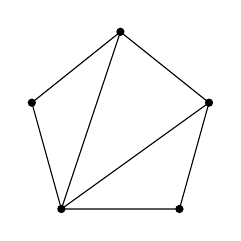
\begin{tikzpicture}[scale=0.75]
        \draw (0,0) -- (2,0) -- (2.5,1.8) -- (1,3) -- (-0.5,1.8) -- cycle; % Pentagon
        \draw (0,0) -- (2.5,1.8); % Diagonal 1
        \draw (0,0) -- (1,3); % Diagonal 2
        \foreach \point in {(0,0), (2,0), (2.5,1.8), (1,3), (-0.5,1.8)}{
            \fill \point circle (2pt); % Vertex points
        }
      \end{tikzpicture}

      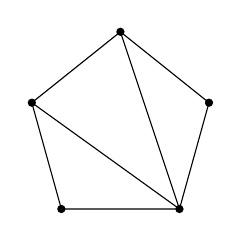
\begin{tikzpicture}[scale=0.75]
        \draw (0,0) -- (2,0) -- (2.5,1.8) -- (1,3) -- (-0.5,1.8) -- cycle; % Pentagon
        \draw (2,0) -- (1,3); % Diagonal 1
        \draw (2,0) -- (-0.5,1.8); % Diagonal 2
        \foreach \point in {(0,0), (2,0), (2.5,1.8), (1,3), (-0.5,1.8)}{
            \fill \point circle (2pt); % Vertex points
        }
      \end{tikzpicture}

      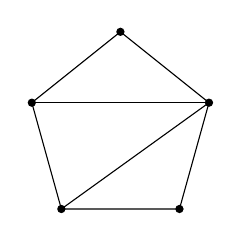
\begin{tikzpicture}[scale=0.75]
        \draw (0,0) -- (2,0) -- (2.5,1.8) -- (1,3) -- (-0.5,1.8) -- cycle; % Pentagon
        \draw (2.5,1.8) -- (-0.5,1.8); % Diagonal 1
        \draw (2.5,1.8) -- (0,0); % Diagonal 2
        \foreach \point in {(0,0), (2,0), (2.5,1.8), (1,3), (-0.5,1.8)}{
            \fill \point circle (2pt); % Vertex points
        }
      \end{tikzpicture}

      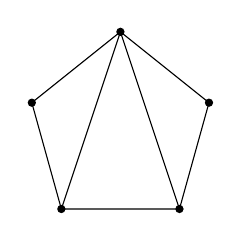
\begin{tikzpicture}[scale=0.75]
        \draw (0,0) -- (2,0) -- (2.5,1.8) -- (1,3) -- (-0.5,1.8) -- cycle; % Pentagon
        \draw (1,3) -- (0,0); % Diagonal 1
        \draw (1,3) -- (2,0); % Diagonal 2
        \foreach \point in {(0,0), (2,0), (2.5,1.8), (1,3), (-0.5,1.8)}{
            \fill \point circle (2pt); % Vertex points
        }
      \end{tikzpicture}

      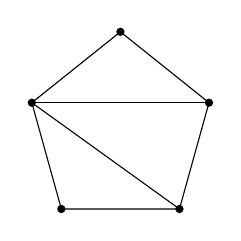
\begin{tikzpicture}[scale=0.75]
        \draw (0,0) -- (2,0) -- (2.5,1.8) -- (1,3) -- (-0.5,1.8) -- cycle; % Pentagon
        \draw (-0.5,1.8) -- (2,0); % Diagonal 1
        \draw (-0.5,1.8) -- (2.5,1.8); % Diagonal 2
        \foreach \point in {(0,0), (2,0), (2.5,1.8), (1,3), (-0.5,1.8)}{
            \fill \point circle (2pt); % Vertex points
        }
      \end{tikzpicture}
    \end{multicols}
  \end{center}

  \begin{proof}
    We proceed by induction on $n$. There is only $C_1 = 1$ way to triangulate a triangle, so the
    base case is done. Suppose $n > 1$. Index the vertices in counter-clockwise order from $0$ to $n
    + 1$, say $v_0, v_1, \dots, v_{n + 1}$. We focus on $v_0$. The the two clockwise most edges
    incident to $v_0$ are $\{v_0, v_1\} \text{ and } \{v_0, v_k\}$, for some $2 \leq k \leq n + 1$.
    Since there are no edges between $\{v_0, v_1\} \text{ and } \{v_0, v_k\}$, $v_0v_1v_k$ form a
    triangle. Removing triangle $v_0v_1v_k$, we get an $k$-gon $v_1v_2\dots v_k$ and an $(n - k +
    3)$-gon $v_kv_{k + 1}\dots v_{n + 1}v_0$. By induction, there are $C_{k - 2}C_{n - k + 1}$ ways
    to triangulate these two polygons, and thus there are $C_{k - 2}C_{n - k + 1}$ triangulations of
    the $(n + 2)$-gon which contains the triangle $v_0v_1v_k$. Therefore, the total number of
    triangulations of an $(n + 2)$-gon is
    \[
      \sum_{k = 2}^{n + 1} C_{k - 2}C_{n - k + 1} = \sum_{i = 0}^{n - 1} C_{i}C_{n - i - 1} = C_n.
    \]
  \end{proof}
\end{homeworkProblem}

\newpage

\begin{homeworkProblem}
  Consider the following variation of counting balanced parentheses. We have a new symbol $*$. Let
  $a_n$ be the number of length $n$ strings consisting of left/right parentheses and $*$ such that
  the result of deleting all of the $*$'s is a balanced set of parentheses ($a_0 = 1$). Let $A(x) =
  \sum_{n\geq0} a_nx^n$. Find polynomials $a(x)$, $b(x)$, $c(x)$ in $x$, not all identically 0, such
  that
  \[ 
    a(x)A(x)^2 + b(x)A(x) + c(x) = 0. 
  \]

  \begin{proof}
    
  \end{proof}
\end{homeworkProblem}

\newpage

\begin{homeworkProblem}
  Let $n$ be a positive integer. Consider the equation
  \[ 
    x_1 + x_2 + \ldots + x_8 = 2n. 
  \]

  For each of the following conditions, how many solutions are there? Give as simple of a formula as
  possible. 

  \begin{enumerate}[(a)]
    \item The $x_i$ are non-negative even integers.
    \begin{proof}
      Let 
      \[
        C_{even} = \{(x_1, \dots, x_8) \mid x_1 + \dots + x_8 = 2n, \, x_i = 2k_i \text{ for some } k_i \in \Z_{\geq 0}\},
      \]
      \[
        C_n = \{(y_1, \dots, y_8) \mid y_1 + \dots + y_8 = n, \, x_i \in \Z_{\geq 0}\}.
      \]
      We show that $C_n \simeq C_{even}$. Define $f: C_{even} \to C_n$ which sends $(x_1, \dots,
      x_8)$ to $(k_1, \dots, k_8)$ and $g: C_n \to C_{even}$ which sends $(y_1, \dots, y_8)$ to
      $(2y_1, \dots, 2y_8)$. Both $f$ and $g$ are obvisouly well-defined. Since 
      \[
        g(f(x_1, \dots, x_8)) = g(k_1, \dots, k_8) = (2k_1, \dots, 2k_8) = (x_1, \dots, x_8),
      \]
      \[
        f(g(y_1, \dots, y_8)) = f(2y_1, \dots, 2y_8) = (y_1, \dots, y_8),
      \]
      $f$ is a bijection, and thus $C_n \simeq C_{even}$. But then we know there are ${n + 7 \choose
      7}$ weak compositions of $n$ with 8 parts, and the result now follows.
    \end{proof}
    \item The $x_i$ are positive odd integers.
    \begin{proof}
      Note that
      \begin{align*}
        \frac{x^8}{(1 - x^2)^8}
        &= \left(x\sum_{a_1 \geq 0} x^{2a_1}\right)\cdots\left(x\sum_{a_8 \geq 0} x^{2a_8}\right) \\
        &= \left(\sum_{a_1 \geq 0} x^{2a_1 + 1}\right)\cdots\left(\sum_{a_9 \geq 0} x^{2a_9 + 1}\right) \\
        &= \sum_{\substack{(k_1, \dots, k_8) \in \Z^8_{\geq 1}, \\ k_i \text{ odd}}} x^{k_1 + \cdots + k_8},
      \end{align*}
      so the number of solutions where all $x_i$'s are positive odd integers are
      \[
        [x^{2n}]\frac{x^8}{(1 - x^2)^8} = [x^{2n - 8}]\frac{1}{(1 - x^2)^8} = [x^{n - 4}]\frac{1}{(1 - x)^8} = {n + 3 \choose 7}.
      \]
    \end{proof}
    \item The $x_i$ are non-negative integers and $x_8 \leq 9$.
    \begin{proof}
      Suppose $x_8 = k$, for some $0 \leq k \leq 9$. Then, there are ${2n - k + 6 \choose 6}$
      solutions, as there are ${2n - k + 6 \choose 6}$ solutions to $x_1 + \cdots + x_7 = 2n - k$.
      Hence, in total, there are $\sum_{k = 0}^9 {2n - k + 6 \choose 6}$ solutions.
    \end{proof}
  \end{enumerate}
\end{homeworkProblem}

\newpage

\begin{homeworkProblem}
  Let $k, n$ be positive integers such that $k \geq n$.
  \begin{enumerate}[(a)]
    \item Show that
    \[
    \sum_{(a_1,\ldots,a_n)} a_1a_2 \cdots a_n = \binom{n+k-1}{k-n},
    \]
    where the sum is over all compositions of $k$ into $n$ parts.
    \begin{proof}
      Note that
      \begin{align*}
        \frac{x^n}{(1 - x)^{-2n}}
        &= xD\left(\sum_{a_1 \geq 0} x^{a_1}\right)\cdots xD\left(\sum_{a_1 \geq 0} x^{a_1}\right) \\
        &= \left(x\sum_{a_1 \geq 1} a_1x^{a_1 - 1}\right)\cdots\left(x\sum_{a_n \geq 1} a_nx^{a_n - 1}\right) \\
        &= \left(\sum_{a_1 \geq 1} a_1x^{a_1}\right)\cdots\left(\sum_{a_n \geq 1} a_nx^{a_n}\right) \\
        &= \sum_{(a_1,\ldots,a_n) \in \Z_{\geq 1}^n} a_1a_2 \cdots a_nx^{a_1 + \cdots + a_n}.
      \end{align*}
      Hence, 
      \[
        \sum_{\substack{(a_1,\ldots,a_n) \in \Z_{\geq 1}^n \\ a_1 + \cdots + a_n = k}} a_1a_2 \cdots a_n = [x^k]\frac{x^n}{(1 - x)^{-2n}} = [x^{k - n}]\frac{1}{(1 - x)^{-2n}} = \binom{n+k-1}{k-n}.
      \]
    \end{proof}
    \item Show that
    \[
    \sum_{(a_1,\ldots,a_n)} 2^{a_2-1}3^{a_3-1} \cdots n^{a_n-1} = S(k, n),
    \]
    where the sum is over all compositions of $k$ into $n$ parts.
    \begin{proof}
      Note that
      \begin{align*}
        F_n(x)
        &= \left(\frac{x}{1 - x}\right)\left(\frac{x}{1 - 2x}\right) \cdots \left(\frac{x}{1 - nx}\right) \\
        &= \left(x\sum_{a_1 \geq 0} x^{a_1}\right)\left(x\sum_{a_2 \geq 0} (2x)^{a_2}\right)\cdots\left(x\sum_{a_n \geq 0} (nx)^{a_n}\right) \\
        &= \left(x\sum_{a_1 \geq 1} x^{a_1 - 1}\right)\left(x\sum_{a_2 \geq 1} (2x)^{a_2 - 1}\right)\cdots\left(x\sum_{a_n \geq 1} (nx)^{a_n - 1}\right) \\
        &= \sum_{(a_1,\ldots,a_n) \in \Z_{\geq 1}^n} 2^{a_2-1} \cdots n^{a_n-1}x^{a_1 + \cdots + a_n}.
      \end{align*}
      Hence,
      \[
        \sum_{\substack{(a_1,\ldots,a_n) \in \Z_{\geq 1}^n \\ a_1 + \cdots + a_n = k}} 2^{a_2-1}3^{a_3-1} \cdots n^{a_n-1} = [x^k]F_n(x) = S(k, n).
      \]
    \end{proof}
  \end{enumerate}
\end{homeworkProblem}

\newpage

\begin{homeworkProblem}
  \begin{enumerate}[(a)]
    \item Give a closed formula for the number of pairs of subsets $S, T$ of $[n]$ such that $S
    \subset T$ (i.e., $S \subseteq T$ and $S \neq T$).
    \begin{proof}
      There are $\binom{n}{k}$ ways to pick a subset of size $k$, and each subset of size $k$ has
      $2^k - 1$ strict subsets. Hence, the total number of $S, T$ pairs is
      \[
        \sum_{k = 0}^n \binom{n}{k}(2^k - 1) = \sum_{k = 0}^n \binom{n}{k}2^k - \sum_{k = 0}^n \binom{n}{k} = (1 + 2)^n - (1 + 1)^n = 3^n - 2^n,
      \]
      by the binomial theorem.
    \end{proof}
    \item Give a closed formula for the number of $k$-tuples of subsets $(S_1, \ldots, S_k)$ of
    $[n]$ such that $\bigcup_{i=1}^k S_i = [n]$.
    \begin{proof}
      Let $a_n$ be the number of $k$-tuples of subsets $(S_1, \ldots, S_k)$ of $[n]$ such that
      $\bigcup_{i=1}^k S_i = [n]$. Put $a_0 = 1$. We show that $a_n = (2^k - 1)^n$ by induction on
      $n$. Given $(S_1, \ldots, S_k)$ such that $\bigcup_{i=1}^k S_i = [n - 1]$, we have to add $n$
      to at least one of the $S_i$'s to ensure $\bigcup_{i=1}^k S_i = [n]$. Since for each such
      $k$-tuple there are $2^k - 1$ ways to do so, we get
      \[
        a_n = (2^k - 1)a_{n - 1} = (2^k - 1)^n,
      \]
      by induction.
    \end{proof}
  \end{enumerate}
\end{homeworkProblem}

\newpage

\begin{homeworkProblem}
  Give a closed formula for the number of $k$-tuples of subsets $(S_1, \ldots, S_k)$ of $[n]$ such
  that $S_i \subseteq S_{i+1}$ for $i = 1, \ldots, k - 1$.

  \begin{proof}
    Notice that the first appearance of any $j \in [n]$ in the tuple determines $j$'s existence in
    all $S_i$'s, as all subsequent sets in the tuple would also contain $j$. Since each $j \in [n]$
    can either first appear in one of the $k$ sets or never appear, there are $k + 1$ choices for
    each element in $[n]$, and thus there are $(k + 1)^n$ $k$-tuples of subsets $(S_1, \ldots, S_k)$
    of $[n]$ such that $S_i \subseteq S_{i+1}$.
  \end{proof}
\end{homeworkProblem}

\newpage

\begin{homeworkProblem}
  What is the total number of parts of all compositions of $k$?

  \begin{proof}
    The possible number of parts of a composition of $k$ is anywhere between $n = 1$ to $n = k$, so
    the total number of parts of all compositions is
    \begin{align*}
      \sum_{n = 1}^k \binom{k - 1}{n - 1}n
      &= \sum_{n = 0}^{k - 1} \binom{k - 1}{n}(n + 1) \\
      &= \sum_{n = 1}^{k - 1} \binom{k - 1}{n}n + \sum_{n = 0}^{k - 1} \binom{k - 1}{n}.
    \end{align*}
    Note that
    \[
      (k - 1)(x + 1)^{k - 2} = D(x + 1)^{k - 1} = \sum_{n = 1}^{k - 1} \binom{k - 1}{n}nx^{n - 1}.
    \]
    Hence,
    \[
      \sum_{n = 1}^k \binom{k - 1}{n - 1}n = (k - 1)(1 + 1)^{k - 2} + (1 + 1)^{k - 1} =  (k + 1)2^{k - 2}.
    \]
  \end{proof}
\end{homeworkProblem}

\newpage

\begin{homeworkProblem}
  Fix an integer $k \geq 2$. Call a composition $(a_1, \ldots, a_n)$ of $k$ doubly even if the
  number of $a_i$ which are even is also even (i.e., there could be no even $a_i$, or $2$ of them,
  or $4$, etc.). Show that the number of doubly even compositions of $k$ is $2^{k-2}$.

  \begin{proof}
    Let $E$ be the set of doubly even compositions of $k$, and $C$ be the set of compositions of $k
    - 1$. We show that $E \simeq C$. Define $f: E \to C$ as
    \[
      f(a_1, \ldots, a_n) = \begin{cases}
        (a_1, \ldots, a_n - 1), & \text{if } a_n > 1 \\
        (a_1, \ldots, a_{n - 1}), & \text{if } a_n = 1 \\
      \end{cases}.
    \]
    On the other hand, define $g: C \to E$ as
    \[
      g(a_1, \ldots, a_n) = \begin{cases}
        (a_1, \ldots, a_n, 1), & \text{if } (a_1, \ldots, a_n) \text{ is doubly even} \\
        (a_1, \ldots, a_n + 1), & \text{otherwise}\\
      \end{cases}.
    \]
    Note that $f$ is obviously well defined. Let $(a_1, \ldots, a_n) \in C$. If $(a_1, \ldots, a_n)$
    is doulby even, then $(a_1, \ldots, a_n, 1)$ is also doubly even. If $(a_1, \ldots, a_n)$ is
    not doulby even, then $(a_1, \ldots, a_n + 1)$ is doubly even, as incrementing $a_n$ by 1 either
    increase or decrease the amount of even numbers in the tuple by 1. Hence, $g$ is also
    well-defined. 

    Since 
    \[
      g(f(a_1, \ldots, a_n)) = \begin{cases}
        (a_1, \ldots, a_{n - 1}, 1), & \text{if } a_n = 1 \\
        (a_1, \ldots, (a_n - 1) + 1), & \text{if } a_n > 1 \\
      \end{cases} = (a_1, \ldots, a_n),
    \]
    \[
      f(g(a_1, \ldots, a_n))= \begin{cases}
        (a_1, \ldots, a_n), & \text{if } (a_1, \ldots, a_n) \text{ is doubly even} \\
        (a_1, \ldots, (a_n + 1) - 1), & \text{otherwise}\\
      \end{cases} = (a_1, \ldots, a_n),
    \]
    $f$ and $g$ are inverses of each other, and thus $E \simeq C$. Hence, the number of doubly even
    compositions of $k$ is equal to the number of compositions of $k - 1$, which is $2^{k - 2}$.
  \end{proof}
\end{homeworkProblem}

\newpage

\begin{homeworkProblem}
  Let $F(n)$ be the number of set partitions of $[n]$ such that every block has size $\geq 2$. Prove
  that
  \[ 
    B(n) = F(n) + F(n + 1),
  \]
  where $B(n)$ is the $n$th Bell number.

  \begin{proof}
    Let $P$ be the set of all partitions of $[n]$, $A_k$ be the set partitions of $[k]$ such that
    every block has size $\geq 2$, and let $S$ be the set of partition of $[n]$ which contains at
    least a singleton. It is obvious that $P = A_n \sqcup S$ and $|A_n| = F(n)$. It remains to show
    that $|S| = F(n + 1)$. 
  
    Define $f: S \to A_{n + 1}$ which puts all singletons of a partition into the same block as $n +
    1$. On the other hand, define $g: A_{n + 1} \to S$ which breaks the block containing $n + 1$
    into singletons and removes $n + 1$. 

    Let $p, p' \in S$, say $p = p' = \{b_1, \ldots, b_l, \{s_1\}, \ldots, \{s_k\}\}$, where $|b_i|
    \geq 2$. Then,
    \[
      f(p) = f(p') = \{b_1, \ldots, b_l, \{s_1, \ldots, s_k, n + 1\}\} \in A_{n + 1},
    \]
    so $f$ is well-defined.

    Now suppose $q, q' \in A_{n + 1}$, say $q = q' = \{b_1, \ldots, b_l, \{s_1, \ldots, s_k, n +
    1\}\}$. Note that each block in $q, q'$ has size at least 2. Then,
    \[
      g(q) = g(q') = \{b_1, \ldots, b_l, \{s_1\}, \ldots, \{s_k\}\},
    \]
    which contains at least one singleton, and thus $g$ is well-defined.

    Since
    \[
      g(f(p)) = g(\{b_1, \ldots, b_l, \{s_1, \ldots, s_k, n + 1\}\}) = \{b_1, \ldots, b_l, \{s_1\}, \ldots, \{s_k\}\} = p,
    \]
    \[
      f(g(q)) = f(\{b_1, \ldots, b_l, \{s_1\}, \ldots, \{s_k\}\}) = \{b_1, \ldots, b_l, \{s_1, \ldots, s_k, n + 1\}\} = q,
    \]
    $f$ and $g$ are inverses of each other, and so $S \simeq A_{n + 1}$.

    But then $|S| = |A_{n + 1}| = F(n + 1)$, and the result follows.
  \end{proof}
\end{homeworkProblem}

\end{document}